\chapter{\appstract{}}\label{chap:appstract}

\section*{Summary}
Web applications are at the cornerstone of modern society.
Web applications are made for humans, yet in many situations we need to automate or monitor interactions with these applications. Such situations include web data extraction, web analytics or web testing.

As soon as the need to scale a solution on multiple web applications in the wild arise, state-of-the-art research in web-related fields often require clever heuristics to compensate for the lack of abstract model.
We argue that a considerable amount of research in a variety of web-related fields can hugely benefit from a universal abstraction inference solution.

We introduce \appstract{}, a solution allowing to infer an abstraction model on any web application with almost no human intervention. 

\section{Introduction}\label{appstract:sec:introduction}
Web applications are often perceived by end-users as online systems exposing a limited set of views, concepts, and related actions.
% As humans, we see a web application as composed of a relatively limited amount of views exposing a limited amount of potential actions. 
From a user perspective, an online shop---like Amazon---mainly offers to search and list products, while clicking on a given product brings us to its details view. 
From a machine perspective, like a bot, navigating the same web application will be perceived as crawling thousands of unique pages, exposing unrelated content and seemingly unique actions.

This inability of a machine to understand the navigation model of a web application, like a user intuitively does, makes it very hard to automate interactions with web applications.
Typically, research topics benefiting from more intuitive navigation include:
\begin{inparaenum}[\it (a)]
    \item \emph{web data mining} to automatically extract, de-noise, and structure data from web pages,
    \item \emph{web testing} to generate, maintain, repair, and augment tests on web applications, and
    \item \emph{web analytics} to report on how users interact with the web application.
\end{inparaenum}

While there is a considerable amount of existing literature, notably in the fields of data mining~\cite{Zhai2005WebAlignment, ArasuExtractingPages, Crescenzi2001RoadRunner:Sites, Sarawagi1996InformationExtraction, ChaudhariTemplatePages, MiaoExtractingClustering}, most of the existing works are highly specific and do not provide adequate insights to build an application-wide understanding of a navigation model.

In particular, state-of-the-art approaches focus on either extracting data within a page (so-called, \emph{intra-page} extraction) or across two pages (\emph{inter-page} extractions). 

For example, Miao~\textit{et~al.}~\cite{MiaoExtractingClustering} clusters full tag paths---\emph{i.e.}, \texttt{/html/body/div[2]/em}---to detect repeating occurrences of a template within a page.
This allows their approach to extract what is usually called \emph{records} in a web page (\emph{e.g.}, a single product card in a product list).
This is an example of what we categorize as \emph{intra-page abstraction}.

\emph{Inter-page abstraction} solutions usually try to detect templates of a webpage or to learn a wrapper by studying two different instances of the same template.
That is what is done by the state-of-the-art algorithms, like EXALG~\cite{ArasuExtractingPages} and \textsc{RoadRunner}~\cite{Crescenzi2001RoadRunner:Sites}.
However, none of these approaches provide any insight to take into account the intra-page variability.

In this chapter, we thus propose an unsupervised approach to infer the navigation model of a whole web application that we call an \textit{appstraction}.
The \textit{appstraction} of a web application aims at delivering actionable insights: it allows a machine to understand application states (\emph{e.g.}, product pages, blog page), as well as elements within states (\emph{e.g.}, product title, price), hence guiding the information extraction process, as well as identifying relevant navigation actions.
The \textit{appstraction} process aims to abstract away the natural variability of web pages into a canonical model built as a compact tree of \emph{template pages} and \emph{template elements}.
Our unsupervised approach assumes that even web applications with billions of pages will build on a limited set of template pages, thus making it possible to infer these generative templates from a dataset of visited pages.
To achieve this, our approach---named \textsc{\appstract{}}---builds on three stages:
\begin{inparaenum}
    \item \textit{web page clustering} to group instances of related web pages,
    \item \textit{intra-page abstraction} to extract repeating patterns within each cluster of pages, and
    \item \textit{inter-page abstraction} to capture repeating patterns across clusters.
\end{inparaenum}

We empirically demonstrate that our \emph{appstraction} succeeds to generate application-wide locators that can be used to support semantic guidance across multiple pages of any web application.

The remainder of this chapter is therefore organized as follows.
Section~\ref{appstract:sec:related} introduces the required background and related works in this area.
Section~\ref{appstract:sec:appstract} presents the design and implementation of \textsc{\appstract{}}, while Section~\ref{appstract:sec:evaluation} reports on an evaluation of the perceived accuracy of \textsc{\appstract{}}.
Finally, Section~\ref{appstract:sec:conclusion} concludes.

\section{Background \& Related Works}\label{appstract:sec:related}
In this section, we present several studies across different research fields that offer partial solutions to the general problem of web application abstraction inference. 
Throughout this chapter, we consider a subset of the Amazon web application as a running example.
In particular, we focus on two related page templates: the product details and product list pages (cf. Figure~\ref{fig:amazon}).

\begin{figure*}[ht]
  \centering
  \begin{subfigure}{.35\textwidth}
    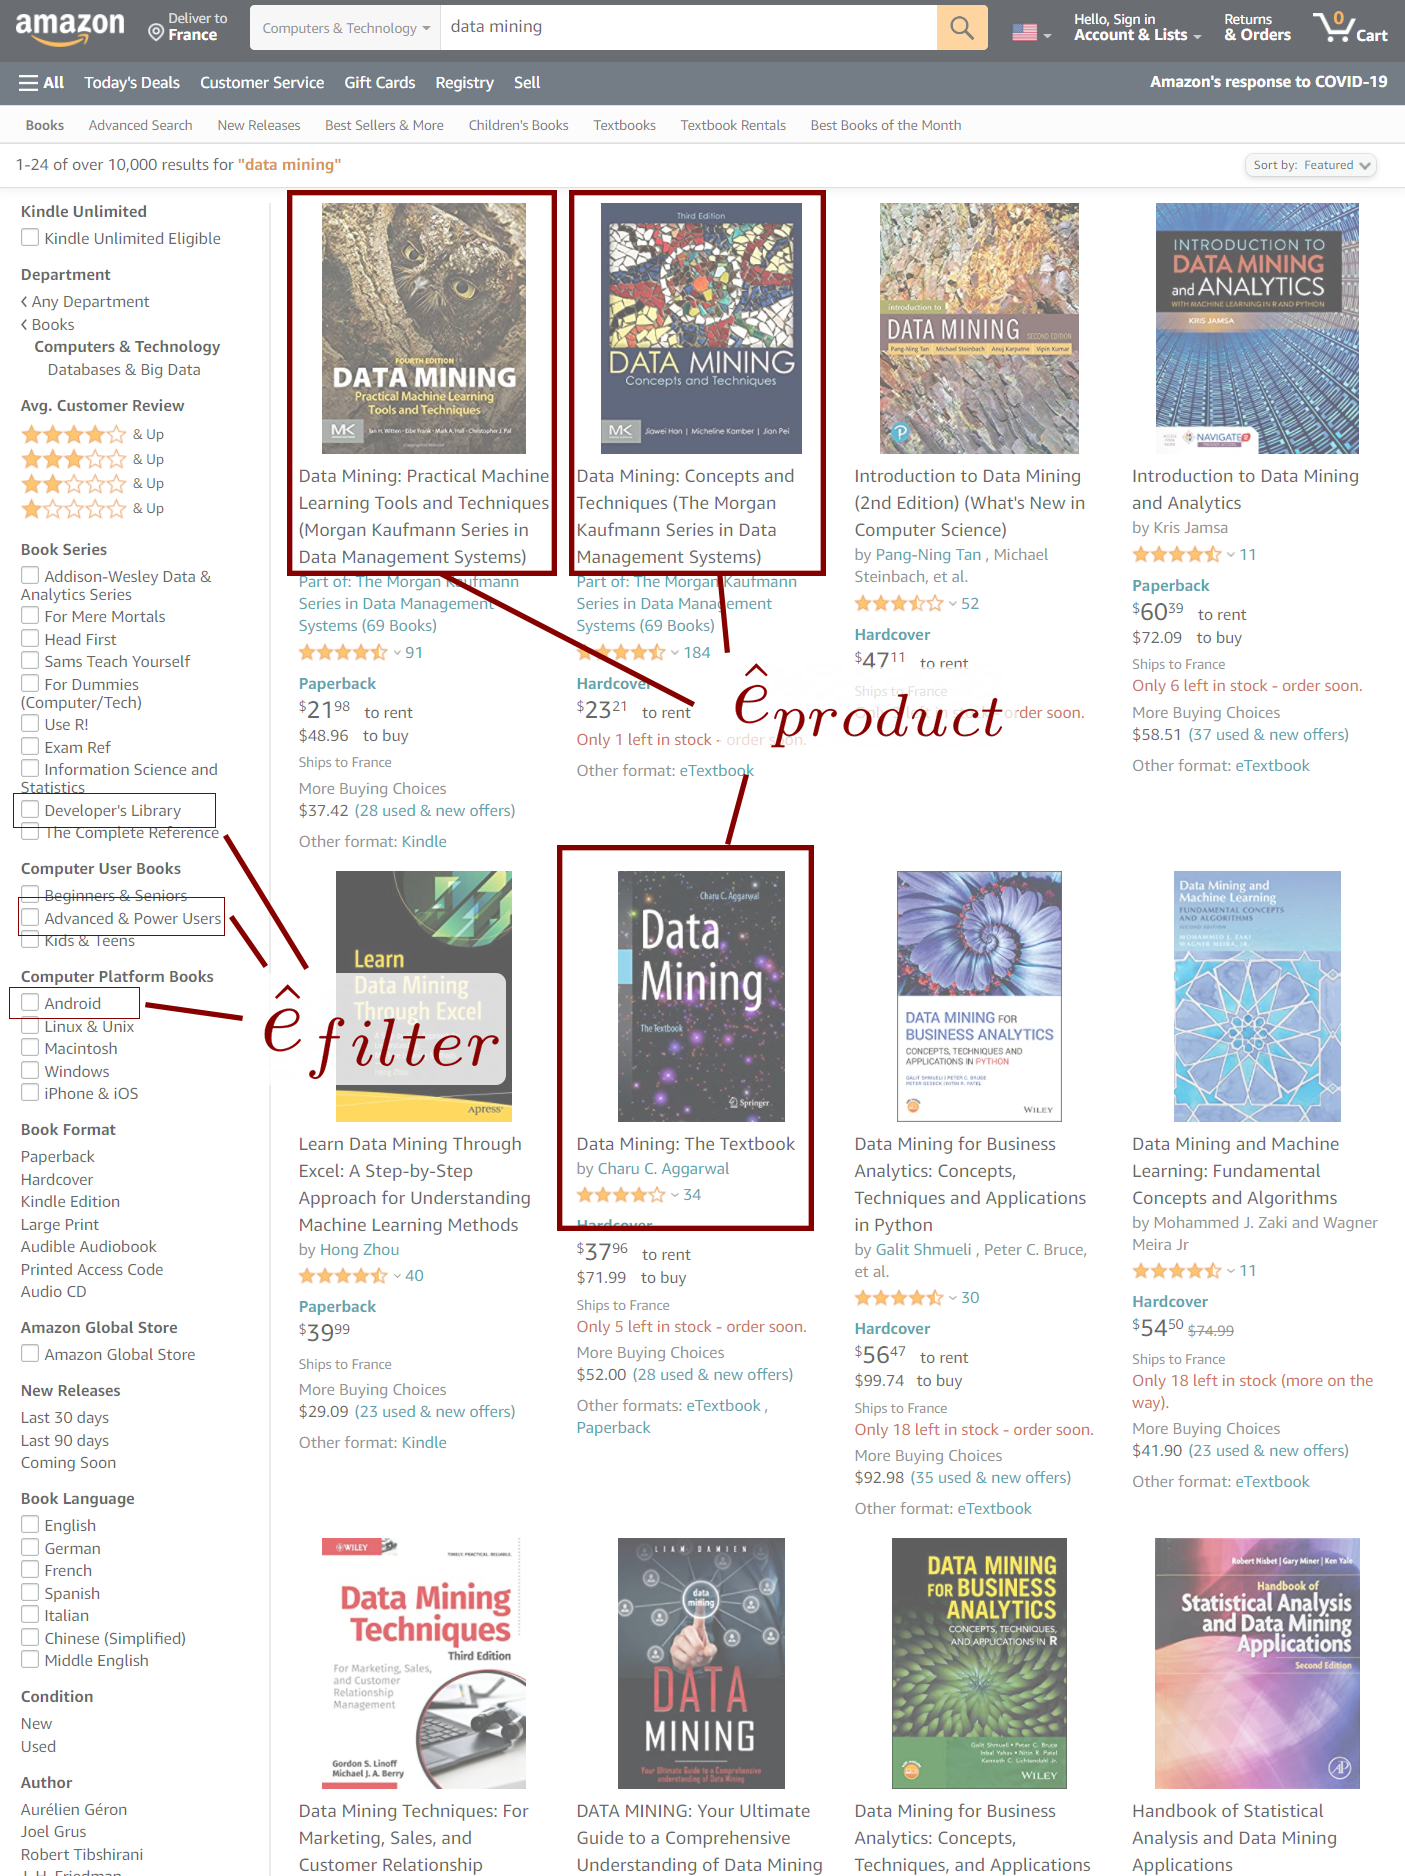
\includegraphics[width=\linewidth]{appstract/amazon_a.png}
    \caption{Sample page from cluster $list$.}
    \label{fig:amazon_a}
  \end{subfigure}
  \hspace{.1\textwidth}
  \begin{subfigure}{.35\textwidth}
    
\includegraphics[width=\linewidth]{appstract/amazon_b.png}
    \caption{Sample page from cluster $product$.}
    \label{fig:amazon_b}
  \end{subfigure}
  \caption{Screenshots illustrating some elements $\hat{e}_{\lambda}$ included in the template pages $\hat{p}_{list}$ and $\hat{p}_{product}$ of 2 distinct clusters.}
  \label{fig:amazon}
\end{figure*}

\subsection{Data Extraction}
The role of a web page is mainly to \emph{present} a subset of the information it has access to in a certain way.
All data extraction solutions attempt to separate the information from its presentation---\emph{i.e.}, the template.
The process of data extraction is thus a form of abstraction of an application: instead of viewing the different pages as a multitude of unrelated blobs of HTML, the application is seen as a limited set of templates that consistently presents various information.
The process of information extraction is thus closely related to our \emph{appstraction} objectives and our approach is highly inspired by the ideas behind data extraction. 

Following the classification made by a survey on data extraction~\cite{Chang2006ASystems}, most existing literature on data extraction can be classified according to the levels of supervision needed to extract the data:
\begin{compactitem}
    \item \emph{(semi-)supervised approaches} where the user inputs more or less detailed directions to describe to how to extract data~\cite{Barish2000TheaterLoc:Applications,Huang2000ExtractingWEB,Levy1996QueryingDescriptions,Muslea1999ExtractionSurvey,Gottlob2004Logic-basedExtraction,Gottlob2004MonadicExtraction,Hsu1998GeneratingWeb},
    \item \emph{unsupervised approaches} where data is automatically extracted by analysing recurring patterns~\cite{Crescenzi2001RoadRunner:Sites,ArasuExtractingPages,Liu2003MiningPages,Wang2002WrapperDiscovery,Wang2002WrapperDiscovery}.
\end{compactitem}

Supervised approaches are usually qualified as "wrapper-based".
The idea of wrapper-based data extraction is to consider the set of web pages containing the data to extract as an unstructured (or semi-structured) database and build a query language (and its query engine) to query the desired data.

In this chapter, we focus solely on \emph{unsupervised approaches}.
These approaches rely on the assumption that even though there are a lot of different pieces of information exposed by an application, the same type of information will always be structured in the same way.
For example, on the product list page of an online shop, each product will be structured in a similar fashion (\emph{e.g.}, product name, price, description).
In this context, we distinguish two families of unsupervised approaches: \emph{intra-page} and \emph{inter-page} data extraction.
One should note that \emph{intra-page} data extraction is usually referred as \emph{record extraction}~\cite{Chang2006ASystems,DeReis2004AutomaticDistance}. 

\emph{Intra-page data extraction} refers to the extraction of data within a page.
For example, in the case of the Amazon page presented in Figure~\ref{fig:amazon_a}, an intra-page data extraction solution, such as MDR~\cite{Liu2003MiningPages}, relies on the topology of the DOM tree and string matching to detect data regions $\hat{e}_{product}$ within a single page.
As is always the case when attempting to extract data in an unsupervised way, MDR can only detect data regions if at least two of these regions are present on the page.
This is a necessary condition since all unsupervised algorithms must rely on some kind of pattern discovery to detect data regions.

\emph{Inter-page data extraction} refers to the extraction of data across several pages.
In particular, all existing algorithms apply to pages that are assumed to belong to the same template (\emph{e.g.}, two Amazon product pages).
The idea is then to use the similarity between the two pages to understand what is common and what has changed between the two pages.
The parts that changed are then assumed to be data, while the common part has to do with its presentation (\emph{template}).
To compare these pages, one solution~\cite{DeReis2004AutomaticDistance} uses a modified version of the most popular general tree matching solution: \emph{tree edit distance}.
In the inter-page abstraction part of our approach, we also use a tree matching solution but not the same one.

The challenge of data extraction presented above is very similar to that of our \emph{appstraction} objective. However, it differs in a few important points:
\begin{enumerate}
    \item while data extraction focuses on extracting data, we try to abstract any kind of variability.
    For example, in Figure~\ref{fig:amazon_a}, a data extraction solution should not attempt to extract the $\hat{e}_{filter}$ template elements, as they do not represent data.
    \item several data extraction studies are focused on how to infer a schema of the extracted data (\emph{e.g.}, relational schema~\cite{ArasuExtractingPages,NestorovExtractingData})), which we are not interested to do in the context of \emph{appstraction}, and
    \item most importantly, to the best of our knowledge, no previous work has attempted to extract data throughout a whole web application (combining both inter-page and inter-page abstraction).
\end{enumerate}

\subsection{Web Testing}
Web testing covers a large body of research that encompasses various themes, such as test generation, test coverage, or test robustness.
We claim that, essentially, the main challenge of web testing comes from the lack of abstract understanding of the application under study and most works in this field have to resort to ingenious ideas to compensate for this lack of an abstract model.

\paragraph{Test Robustness}
One of the main challenges of web testing encountered by the industry is test breakage: tests written for a given version of a web application break when the application evolves.
For example, let us consider a testing script that applies to a web page $D$.
One part of the script instructs to click on a given button $e$ on the page $D$.
To locate $e$, scripts usually use xPath or CSS selector to build what is called a \emph{locator} $l_e$. 
Breakage can then happen when a new version $D'$ of the page $D$ is published.
Most of these breakage are locator based~\cite{Hammoudi2016WhyBreak}: the locator $l_e$ that successfully located $e$ on $D$ does not locate the matching element $e'$ in $D'$. 
To solve this problem, some attempt to automatically generate more robust locators relying on the structure of the tree~\cite{Leotta2016spanLocators, Leotta2021Sidereal:Testing, Yandrapally2014RobustClues, Bajaj2016SynthesizingLocators} while other works offered solutions to repair broken locators~\ref{chap:erratum}.

In particular, The \erratum{} approach~\ref{chap:erratum} achieves high accuracy specifically thanks to a more holistic stance: instead of looking at individual locators independently, the approach considers the page as a whole using a similar technique to the \emph{inter-page abstraction} part of our \emph{appstraction}.

The "locator" problem is a more specific instance of the web application abstraction: the breakage happens because when a machine sees a multitude of different pages (\emph{e.g.}, different versions), a human perceives a single page template with slight differences and thus comes to expect the locators on $D$ should naturally work on $D'$. 

In the present work, we go beyond \erratum{}~\ref{chap:erratum} on the generalization scale and create "locators" that are valid through all pages of a web application.

\paragraph{Test Generation}
Automatic test generation is a domain of research that studies different approaches to automatically generating tests. Most test generation techniques rely on an abstraction of the application called a navigational model. A navigational model of a web application describes the different states an application can be in and the transitions between them~\cite{mesbah2009invariant}.

There exist many approaches to take advantage of this navigational model. The goal of these techniques is to generate the minimum amount of tests that covers a maximum of the application's behavior given a navigation model~\cite{leveau2022fostering, mesbah2009invariant, yuan2007using, biagiola2019diversity}

We are particularly interested in the generation of the underlying navigational model.
The navigational model can be written manually, for example, Leveau and al.~\cite{leveau2022fostering} developed a whole Domain Specific Language to describe this navigational model. 
It can also be generated. The only approach we managed to find that generates a navigational model is APOGEN~\cite{stocco2017apogen}. APOGEN is quite close in spirit to our APPSTRACT solution. The idea of APOGEN is not originally to create a navigational model but to create \textit{page objects}. However, it has been used as a way to generate a navigational model~\cite{biagiola2019diversity}. APOGEN crawls, clusters, and then analyses the different clusters of a web application to generate page objects. The main difference with our approach is that APOGEN is heavily based on the analysis of links to understand how different pages interact with one another and most importantly, it does not include any \textit{intra-page abstraction}.

\subsection{Web Analytics}
Web analytics deals with the analysis of the user behavior on a given web application.
A lot of studies have been published on the subject since the popularisation of the web. However, most works are applied in controlled environments where the ability to automatically infer an abstract model of an application is not needed. For example, some research focuses solely on mouse movements~\cite{guo2008exploring, yamauchi2013mouse} or focuses on a given search engine and tries to analyze behavior to optimize search results~\cite{agichtein2006learning, agichtein2006improving}.
Research that does rely on a certain model of an application usually uses an \textit{url-based} model. While the first research works on the subject, at the beginning of the web, could use simple logs of visited urls~\cite{gunduz2003web, mobasher2001effective, sarukkai2000link}, modern web applications are generally much more complex with virtually unlimited amounts of URLs dynamically generated making it hard to reason about unprocessed logs of visited URLs.
To tackle this challenge, recent work on web browsing behavior uses a variety of techniques to encode URLs like Recurrent neural network~\cite{Ou2021ModelingSide} so that several strictly different URLs that refer to the same template page will have similar encodings. While using URL-based encoding to create an abstract model of a web application can help abstract relationship \textit{between} pages (given that they contain enough information which depends on the application), it will not provide the \textit{intra-page} abstraction that we need to obtain meaningful encodings within pages.

\section{\appstract{}}\label{appstract:sec:appstract}
\subsection{Abstracting a Web Application}
This section starts by defining the notions of \emph{application} and \emph{application abstraction} we assume, before discussing the challenges of inferring such defined abstractions.

\begin{defn}[\em Application]
A web application $A$ is a set of web pages $\{p \in A\}$, where every page $p$ is captured by a \emph{Document Object Model} (DOM).
\end{defn}

The number of web pages $\|A\|$ can be very high and keep rising with time (\emph{e.g.}, Amazon products or blog posts).
In addition, we consider that any mutation of a web page (even if the URL does not change) is considered a new page.
Obviously, from a human perspective, a web application is much more than a collection of pages (\emph{e.g.}, the pages are linked, the application has different features usable by different users), but we choose to take the perspective of a machine, for which an application is perceived as a set of visited web pages.
% 
As a DOM of a page $p$ is a tree, we represent it as a tuple $\langle N(p), par \rangle$ where $N(p)$ is the set of elements (or nodes) in $p$ and $par: N(p) \to N(p)$ is the parent function that associates a DOM node with its parent.
To lighten the notations, we write $e \in p$ to describe an element $e$ in a page $p$, instead of writing $e \in N(p)$.

\begin{defn}[\em Application abstraction]
The abstraction of a web application $A$ is a tuple $\langle\hat{A}, T_{\hat{A}}\rangle$ where \emph{i)} $\hat{A}$ is the set of template pages and each page $\hat{p} \in \hat{A}$ contains template elements $\hat{e} \in \hat{p}$ and \emph{ii)}:
\begin{align}
  \label{eq:1}
  \begin{split}
    \forall p \in A, T_{\hat{A}}(p) & = \langle\hat{p}, T_{\hat{p}}\rangle \\
    \text{and } \forall e \in p, T_{\hat{p}}(e) & = \langle\hat{e}\rangle
  \end{split}
\end{align}\end{defn}

In other words, the abstraction of a web application $A$ is a set of template pages (\emph{e.g.}, product page, list page) and a function that allows mapping any page from $A$ to its corresponding template, and every element within the page to the corresponding element in the template page.
This mapping is completed by two functions:
\begin{enumerate}
\item $T_{\hat{A}}: A \to \hat{A}$ is the template function that takes any page $p \in A$ and returns the matched \emph{template page} $\hat{p} \in \hat{A}$, and
\item $T_{\hat{p}}: N(p) \to N(\hat{p})$ is a function that takes any element $e \in p$ and returns the matched element in the template $\hat{e} \in \hat{p}$.
\end{enumerate}

Additionally, we also use:
\begin{itemize}
  \item $T^{-1}_{\hat{A}}(\hat{p}) \subset A$ as the set of pages $p \in A$, such that $T_{\hat{A}}(p) = \hat{p}$, and 
  \item $T^{-1}_{\hat{p}}$ as the inverse function of $T_{\hat{p}}$.
\end{itemize}
These notations allow us to easily refer to the instance pages/elements of a given template page/element.

Figure~\ref{fig:amazon} depicts a theoretical application of the appstraction to 2 web pages crawled from Amazon.
For each related clusters of similar web pages, the $T_{\hat{A}}$ function will return either template page $\hat{p}_{list}$ or $\hat{p}_{product}$.
Then, for each clustered web page, each web element can be mapped to its corresponding template element (\emph{e.g.}, $\hat{e}_{title}$, $\hat{e}_{product}$) using the $T_{\hat{p}}$ function.

Please note that our \emph{appstraction} process does not intend to label template pages or elements.
Thus, our references to $\hat{p}_{list}$ or $\hat{e}_{product}$ should be understood as a \emph{global unique identifier} (GUID) capturing a class of pages and elements within and across clusters.
% , it is solely for pedagogical purpose: while a good appstraction of the application would be able to map all instances of $\hat{e}_{product}$ to the same template element, we do not provide any solution to infer the label ("product" in this case) of this template element.

\subsection{Building an Abstraction}

\begin{figure*}[ht]
  \centering
  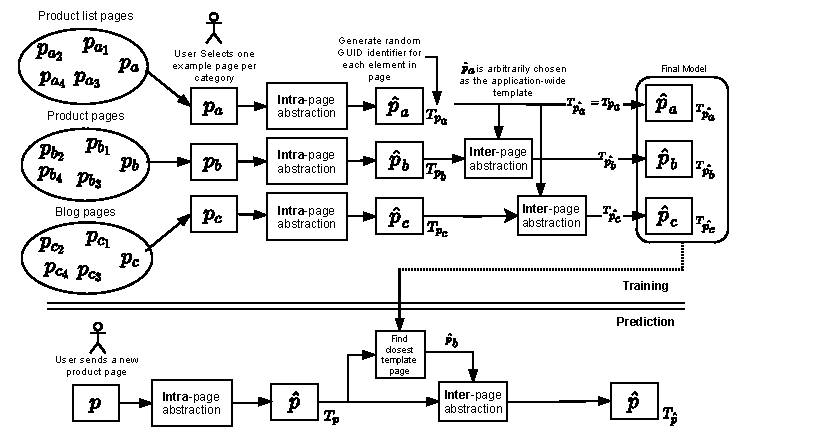
\includegraphics[width=0.8\linewidth]{appstract/explanations/appstract_overview}
  \caption{Overview of the two stages of the \emph{appstraction} process: \emph{learning} and \emph{prediction}. The identifier map of $p$ noted $T_p$ associates an identifier to each element of $p$. The identifiers are first randomly generated, then merged to existing maps during inter-page abstraction. The prediction phase produces an identifier map $T_{\hat{p}}$ in which each original element of $p$ is associated with an application-wide identifier.}
  \label{fig:appstract_overview}
\end{figure*}

To abstract the web page $p$ into its \emph{appstraction} $A_p$, we operate at two levels:
\begin{enumerate}
  \item \textit{intra-page abstraction} to extract repeating patterns of elements within a cluster of web pages, and
  \item \textit{inter-page abstraction} to group repeating patterns of elements across template pages.
\end{enumerate}

This bi-level abstraction process combines two steps: \emph{learning} and \emph{prediction}, as depicted in Figure~\ref{fig:appstract_overview}.
% There are two stages to the overall appstraction process: \emph{training} and \emph{prediction}.
% Figure~\ref{fig:appstract_overview} describes how both stages contribute to build an application abstraction.
% 
In this section, we first overview the abstraction process by considering intra- and inter-page abstractions as black boxes. 
In the following sections, we provide an in-depth description of individual-level abstraction techniques.

\paragraph{Learning}
The objective of the learning phase is to build a model of the application that will deliver accurate predictions.
The upper part of Figure~\ref{fig:appstract_overview} describes how intra- and inter-page abstractions are used to build this model.

Before any abstraction, the application is perceived as a set of related pages.
The first step is thus to organize these pages into clusters, each cluster representing a template page (\emph{e.g.}, product page).
To do this, any clustering algorithm could be used and, in this chapter, we consider the clustering part as out of scope as we focus on the actual abstraction process.
The learning approach thus starts with the user picking one example page per template.

Each template page goes through intra-page abstraction.
The intra-page abstraction takes a DOM tree $p$ as input and returns a \textit{template} as output.
A \textit{template} is a tuple $t = \langle \hat{p}, T_p \rangle$ where $T_p$ is the identifier map that maps every element from the original tree $p$ to a global identifier. After the intra-page abstraction, $\hat{p}$ typically contains much fewer elements than $p$ since all repeated patterns have been abstracted away.
The $T_p$ map is a way to keep track of the elements in the original page $p$ after abstraction.
For example, in Figure~\ref{fig:intra} illustrating intra-page abstraction, the identifier map would contain 11 entries, one for each original element in $p$ and 5 distinct values corresponding to the five distinct nodes of $\hat{p}$.

In practice, the values of $T_p$ are \emph{Global Unique Identifiers} (GUID).
Before starting the abstraction process, we transform the page $p$ into a \textit{template} tuple, where the identifier mapping maps every node to a randomly generated GUID.
Each abstraction step will thus transform the input tree and update the associated identifier map.

Once each page has been abstracted at the intra-page granularity, we build a model allowing us to achieve two aspects of inter-page abstraction:
\begin{itemize}
    \item \textit{Template abstraction:} same elements within different instances of a template must have the same identifiers (\emph{e.g.}, the title of a product on different product pages)
    \item \textit{Cross-template abstraction:} same elements within different pages (regardless of templates) should have the same identifiers. (\emph{e.g.}, menu link that appears on all template pages)
\end{itemize}

To achieve cross-template abstraction, we arbitrarily select one template to represent the whole application ($\langle \hat{p}_a, T_{p_a} \rangle$ in Figure~\ref{fig:appstract_overview}) we call this template the \textit{mother template}.
All other template pages are then inter-page abstracted against the mother template. 
The inter-page abstraction function takes two templates: a reference template and a query template. It then returns one template in which the values of the identifier map have been updated to match the reference template.

The final model is obtained after applying intra-page abstraction between the mother template and all other pages.
The final model is simply a set of $n$ templates where each template is a tuple $\langle \hat{p}, T_{p} \rangle$.

\paragraph{Prediction}
During the prediction phase described in the bottom part of Figure~\ref{fig:appstract_overview}, the user sends a previously unseen page and \textsc{\appstract{}} returns the mapping between each element $e$ of the page and the \textit{id} of the associated template element $\hat{e}$.

To do so, \textsc{\appstract{}} first applies intra-page abstraction to create an abstracted DOM tree $\hat{p}$, then applies the tree matching algorithm at the core of the inter-page abstraction between $\hat{p}$ and all templates in the model.
The template page from the model that matches best with $\hat{p}$ is retained (\emph{e.g.}, $\hat{p_b}$ in Figure~\ref{fig:appstract_overview}).

The matching between $\hat{p}$ and the corresponding template is then used to compute the final mapping $T_{\hat{p}}$.

Overall, the user sent a page and received the mapping between each element of the page and the corresponding template element in the corresponding template page.

In the following sections, we describe both intra-page abstraction and inter-page abstraction in more detail.

\subsection{Intra-Page Abstraction}

\begin{figure*}[ht]
  \centering
  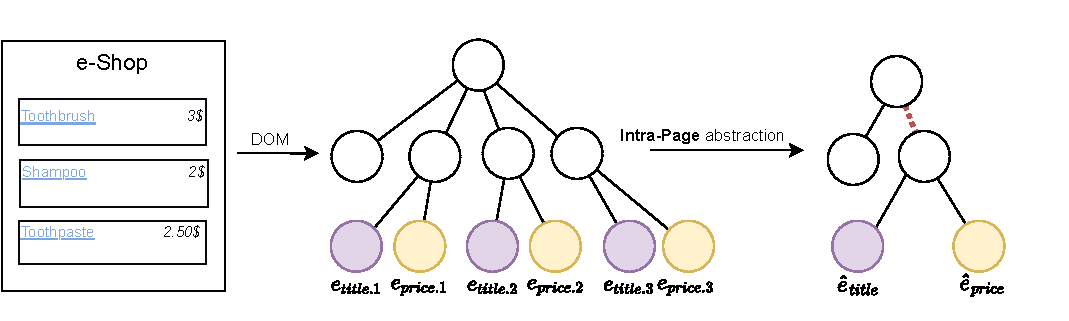
\includegraphics[width=0.8\linewidth]{appstract/explanations/intra}
  \caption{Illustration of Intra-Page abstraction. DOM leaves at the end of repeating branches are tagged and then recursively merged.}
  \label{fig:intra}
\end{figure*}

Intra-page abstraction relies on the detection of repeating patterns within a page. 

Building the intra-page abstraction corresponds to creating the $T_e$ function defined above.
The intra-page abstraction deals with a single page: given an input page $p$, we want to build a template page $\hat{p}$ and a function $T_e$ that maps all the elements $e \in p$  to their corresponding elements $\hat{e} \in \hat{p}$
Overall, the Intra-Page abstraction is done in three steps:
\begin{enumerate}
  \item \emph{Leaf clustering} clusters repeating DOM leaves together,
  \item \emph{Node tagging} propagates information about leaf clusters in all ancestor nodes to prepare for the final step,
  \item \emph{Recursive leaf-group merging} builds the intra-page abstraction by recursively merging branches.
\end{enumerate}

\subsubsection{Leaf Grouping}
In the first step of intra-page abstraction, we attempt to identify groups of leaf nodes that present data of the same type.
To do so, we:
\begin{inparaenum}
  \item build all root-to-leaf paths from the DOM tree,
  \item group all same paths together, and
  \item filter out groups of leaves containing less than a fixed threshold $k$ of elements.
\end{inparaenum}
At the end of this phase, we have a set of leaf groups ($LG$), each containing at least $k$ elements.

The \emph{root-to-leaf} path of a node is the formatted sequence of tags from the root to the node.
For example, on the web page from Figure~\ref{fig:non_recursive_html}, the root-to-leaf path of the element containing the text \emph{price2} is \lstinline{//html/body/div/span/}.

\begin{figure}[ht]
  \centering
  \begin{lstlisting}
    <html>
      <head> <!-- header --> </head>
      <body>
          <div> <!-- content --> </div>
          <div>
              <a href="...">Item1</a>
              <span>price1</span>
          </div>
          <div>
              <a href="...">Item2</a>
              <span>price2</span>
          </div>
      </body>
    </html>
  \end{lstlisting}
  \caption{Web page example to illustrate intra-page abstraction with no nested records}
  \label{fig:non_recursive_html}
\end{figure}

To find leaf groups, we extract all root-to-leaf paths from the DOM tree and group the same ones together
and only keep the groups that contain more than a fixed threshold $k$ of elements.
In example~\ref{fig:non_recursive_html}, assuming $k=2$, it means we have two groups:
\begin{compactenum}
  \item Leaf group 1 (\texttt{//html/body/div/span/}) containing \texttt{price1} and \texttt{price2}, and
  \item Leaf group 2 (\texttt{//html/body/div/a/}) containing \texttt{Item1} and \texttt{Item2}.
\end{compactenum}
In our evaluation, however, this threshold is set to $k=4$.

% Probably to move somewhere else
\paragraph{Limits}
Our grouping method may fail to cluster items correctly in two situations:
\begin{compactitem}
  \item \emph{Over-abstraction}: Items can be clustered together even if they are not of the same type, or
  \item \emph{Sub-abstraction}: Items can be put in different clusters even though a human would put them in the same cluster.
\end{compactitem}
To a certain extent, \emph{sub-abstraction} can be compensated afterwards.
For example, when extracting information, it is common for websites to structure data differently according to the type of exposed products (\emph{e.g.}, regular products or "sponsored" products). 
In this case, using the approach we presented, the two types of products will be classified in different clusters, meaning that if the data is extracted as a table, the prices will be spread in two different columns that the user will be able to easily merge.

The cases of \emph{over-abstraction} are more problematic since it will mean that the associated data has been lost when abstracting the page.

\subsubsection{Node Tagging}
\label{appstract:sec:node_tagging}
At this stage, we have a list of all leaf groups ($LG_1, LG_2...$). 
To be able to recursively merge all leaf groups, we propagate the information that a leaf belongs to a certain group to all ancestors of the leaf using the node-tagging algorithm~\ref{algo:node_tagging}.

\begin{algorithm}
\caption{Intra-Page abstraction: Node Tagging}\label{appstract:alg:intra_tagging}
\begin{algorithmic}[1]
  \Function{createTags}{$LGs = [LG_1, LG_2...]$}
    \Function{tagBranch}{$depth$, $LG$, $e$}
      \State $tag \gets \langle LG, depth \rangle$
      \State $e.tags[tag] += 1$ \Comment{Inc or init $tag$ count of node $e$}
      \State tagBranch($depth + 1$, $LG$, $e.parent$)
    \EndFunction
    \ForAll{$LG \in LGs$}
      \ForAll{$e_{leaf} \in LG$}
        \State tagBranch(0, $LG$, $e_{leaf}$) 
      \EndFor
    \EndFor
  \EndFunction
\end{algorithmic}
\label{algo:node_tagging}
\end{algorithm}

Algorithm~\ref{algo:node_tagging} iterates through all the leaves that belong to a leaf group $LG$ and for each leaf, it recursively tags all the ancestors of the leaf. 
The $tag$ of an element $e$ is the tuple $\langle LG, depth \rangle$ where $LG$ is a leaf group and $depth$ is the number of nodes between $e$ and the leaf from its offspring that belongs to $LG$.
The tag is used to identify nodes that should be merged.

When the algorithm ends, each node $e$ of the DOM tree contains a map $tags$ whose keys are tags and values are integers count. 
Figure~\ref{fig:node_tagging} shows an example result of the node-tagging algorithm on a simple DOM tree. 

\begin{figure}[ht]
  \centering
  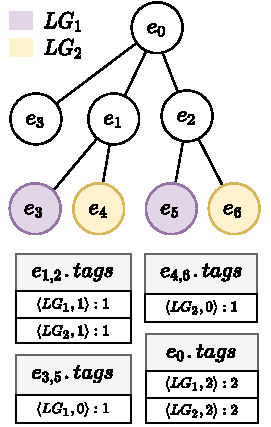
\includegraphics[width=0.5\linewidth]{appstract/explanations/node-tagging}
  \caption{Output of the node-tagging algorithm. Each node is assigned a $tags$ map keeping track of the number of leaf groups in its offspring.}
  \label{fig:node_tagging}
\end{figure}

An important implementation detail: the above algorithm assumes that the $tag$ tuple's hash code will be generated from the value of its components (and not the object's reference)---\emph{i.e.}, two $tag$ tuples containing the same leaf group $LG$ and the same $depth$ should have the same hash code when inserted into the $e.tags$ map (even though the tags will have different addresses in memory since they were created at a different stage of the algorithm).

\subsubsection{Recursive Branch Merging}
\paragraph{Overview}\label{appstract:sec:overview}
The last step of the intra-page abstraction consists in merging all required nodes such that the resulting DOM contains only one node instance of each leaf group. 
Figure~\ref{fig:intra} shows an example of the result obtained after this last step of the intra-page abstraction. 
In the final abstract tree of Figure~\ref{fig:intra}, the red dotted edge connecting the template element $\hat{e}$ to its parent indicates that $\hat{e}$ has a special relationship with its parent, in this case: a 1-to-many relationship.

The algorithm must be recursive because it is possible (and likely) that some leaf groups will have to be merged at different levels of the tree. 
Figure~\ref{fig:intra-use-cases} illustrates this use case: $e_{a1}$ and $e_{a2}$ must be merged first before their ancestor $e_{b1}$ can merge with $e_{b2}$.

\begin{figure}[ht]
  \centering
  \begin{subfigure}{0.4\textwidth}
    \centering
    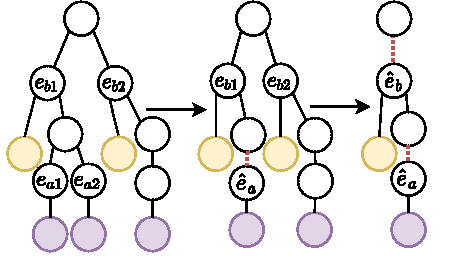
\includegraphics[width=.9\linewidth]{appstract/explanations/intra-recursivity}
    \caption{Nested records}
    \label{fig:nested_records}
  \end{subfigure}
  \begin{subfigure}{0.4\textwidth}
    \centering 
    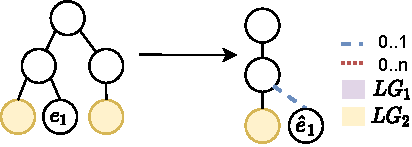
\includegraphics[width=.9\linewidth]{appstract/explanations/intra-optional}
    \caption{Optional elements}
    \label{fig:optional_elements}
  \end{subfigure}
  \caption{Illustrating two important cases our merging algorithm must cover: \emph{nested records} and \emph{optional elements}.}
  \label{fig:intra-use-cases}
\end{figure}

The second case illustrated in Figure~\ref{fig:optional_elements} occurs when merging two nodes even though not all their respective children are merged.
In this case, the inferred abstract node $\hat{e}_1$ is said to have an \textit{optional} relationship with its parent template element---\emph{i.e.}, it only exists as a child node in certain instances of $\hat{e}_1$.
In general, a template element $\hat{e}$ can have many types of relationships with its parent.
In this chapter, we distinguish two relationships:
%% TO revise, it's heavy and probably wrong
\begin{compactitem}
    \item A \emph{zero-to-many relationship} when at least one element from $T^{-1}_e(par(\hat{e})) = par(e_1), par(e_2)...$ has no child element that is an instance of $\hat{e}$ and at least one other element has more than 1,
    \item An \emph{optional (or zero-to-one) relationship} when at least one element from $T^{-1}_e(par(\hat{e})) = par(e_1), par(e_2)...$ has no child element that is an instance of $\hat{e}$ and at least one other element has more than 1.
\end{compactitem}

\paragraph{Algorithm}
Algorithm~\ref{appstract:alg:abstractTree} gives a high level view of the solution.
The function \emph{abstractTree} recursively traverses the tree.
For each node $e$ considered, it checks if $e$ is already abstract using the \emph{isAbstract} function (line \ref{appstract:alg:abstractTree:isAbstract}).
A node is abstract if none of its children need to be merged.
If $e$ is already abstract then it is returned, otherwise, we:
\begin{compactenum}
  \item recursively call the \emph{abstractTree} function on all children of $e$,
  \item group all abstract children by group of tags using \emph{assocGroup} (see paragraph~\ref{par:assocGroup}), and
  \item merge each group of children using \emph{mergeGroup} (see paragraph~\ref{par:mergeGroup})
\end{compactenum}

\begin{algorithm}
\caption{Intra-page abstraction: recursive merge}\label{appstract:alg:abstractTree}
\begin{algorithmic}[1]
  \Function{abstractTree}{$e: Element$}
    \If {isAbstract($e$)}
      \label{appstract:alg:abstractTree:isAbstract}
      \State \Return $e$
    \Else
      \State children $\gets$ $e$.children.map(abstractTree)
      \State children $\gets$ assocGroup(children).map(mergeGroup)
      \State $\hat{e}$ $\gets$ \{ $e$ with $e$.children = children \}
      \State \Return $\hat{e}$
    \EndIf
  \EndFunction
\end{algorithmic}
\end{algorithm}

We describe in details the three functions used in algorithm~\ref{appstract:alg:abstractTree}, namely:
\begin{inparaenum}
  \item \emph{isAbstract},
  \item \emph{assocGroup}, and
  \item \emph{mergeGroup}.
\end{inparaenum}

\paragraph{isAbstract}
The function \emph{isAbstract} checks if an element $e$ is already abstract.
An element $e$ is abstract if none of its offsprings need to be merged.
This information is obtained using the tags computed in previous steps (see Section~\ref{appstract:sec:node_tagging}).

Each tag $tag$ associated to a node $e$ is associated to its tag count $|tag|$.
Using the tag counts, we can then detect if $e$ is abstract: a node $e$ is abstract iff all tag counts are equal to 1.
In this case, it means that no node in the offspring will have to be merged.
For example, in Figure~\ref{fig:node_tagging}, all nodes are abstract except $e_{0}$ since two tags in $e_{0}.tags$ have a tag count of 2.
In practice, it means that some children of $e_{0}$ (in this case $e_{1}$ and $e_{2}$) will have to be merged.

\paragraph{assocGroup}\label{par:assocGroup}
The function \emph{assocGroup} (for associative grouping) groups all the nodes that need to be merged.
To know if two nodes need to be merged, we look at their associated \emph{tags} map.
The merging condition is simple: two nodes should be merged iff they share the same tag.
Below is an example of input/output pair of the \emph{assocGroup} function:
\begin{lstlisting}
    Input:
        A has t1, t2
        B has t2, t3
        C has t3
        D has t4
        E has t4

    Output:
        [A, B, C] -> [t1, t2, t3]
        [D, E] -> [t4]
\end{lstlisting}

In our case, the letters $A$ to $E$ are nodes and $t1$ to $t4$ are tags.

\paragraph{mergeGroup}\label{par:mergeGroup}
The function \emph{mergeGroup} is the core of the recursive merging algorithm.
As an input, it takes a list of abstract nodes---\emph{i.e.}, abstract subtrees---that need to be merged and the set of common tags between the groups of nodes.
The output is the abstract node $\hat{e}$.
The inputs come from the output of the function \emph{assocGroup}, described above, and the abstract node output replaces all children that were merged in the tree, as shown in the \emph{abstractTree} algorithm~\ref{appstract:alg:abstractTree}

The function \emph{mergeGroup} reduces the group list taken as input by repeatedly applying the function \emph{mergeAbstractTrees}.
Algorithm~\ref{appstract:alg:mergeAbstractTrees} describes how the function merges two abstract trees into one.

\begin{algorithm}
\caption{Intra-page abstraction: merge two abstract trees}\label{appstract:alg:mergeAbstractTrees}
\begin{algorithmic}[1]
  \Function{mergeAbstractTrees}{$\hat{e}_1, \hat{e}_2$}
    \State \Comment{Group pairs of children containing the same tags}
    \State pairs, orphans $\gets$ groupPairs($\hat{e}_1$, $\hat{e}_2$)
    \State mergedChildren $\gets$ pairs.map(mergeAbstractTrees)
    \For{$e$ in orphans}
        \State $e$.rel $\gets$ relType.Optional
    \EndFor
    
    \State $\hat{e}$ $\gets$ new Node()
    \State $\hat{e}$.tag = $\hat{e}$.tag
    \State $\hat{e}$.attrs = mergeAttrs($\hat{e}_1$.attrs, $\hat{e}_2$.attrs)
    \State $\hat{e}$.rel = mergeRel($\hat{e}_1$.rel, $\hat{e}_1$.rel)
    \State $\hat{e}$.children = mergedChildren + orphans
    \State $\hat{e}$.tags = \{$\hat{e}_1 \cup \hat{e}_2$ with tag counts set to 1\}
    \State \Return $\hat{e}$
  \EndFunction
\end{algorithmic}
\end{algorithm}

Before diving into the details of the algorithm, it is important to highlight that the inputs of the function \emph{mergeAbstractTrees} are already abstract.
At this stage of the algorithm, we are assured that along the whole branch starting at the root of both nodes sent as parameters, there are never two children belonging to the same cluster---\emph{i.e.}, that needs to be merged.
It means that the algorithm's sole purpose is to recursively merge the two trees between them (and not within).

The function starts by grouping the children of the two nodes into pairs and orphans.
The function \emph{groupPairs} returns two lists: the pairs of nodes that must be merged and the orphan nodes. 
The orphan nodes are the children in $\hat{e_{1/2}}$ that have no corresponding element to be merged within $\hat{e_{2/1}}$, these elements are set as optional using the \emph{rel} (as in relationship) property.

Before merging, we recursively call the function \emph{mergeAbstractTrees} on each pair of nodes returned by \emph{groupPairs}.
Intuitively, the algorithm will stack the calls to \emph{mergeAbstractTrees} until it reaches the leaves of
the trees, then it will merge the groups of leaves and merge their ancestors as the function calls unstack.

Most of the steps described above help compute the \emph{children} property of the abstract node returned by the \emph{mergeAbstractTrees} function.
Other properties of the nodes are also merged: 
\begin{compactdesc}
\item[\emph{rel}:] In case the relationships of the nodes to merge are different, they are merged using the following pattern matching:
\begin{lstlisting}[basicstyle=\small]
  mergeRelTypes :: (RelType,RelType)->RelType
  mergeRelTypes (t1, t2)
      | (t1, t2) when t1 = t2 -> t1
      | (t1, Normal) -> t1
      | (_, ZeroToMany) -> ZeroToMany
      | (Optional, OneToMany) -> ZeroToMany
      | (t1, t2) -> mergeRelTypes (t2, t1)
\end{lstlisting}

\item[\emph{attrs}:] In case the attributes of the nodes to merge are different, they are merged.
To merge the attributes, we select the attributes that are present in both nodes and merge their values using the \emph{Longest Common Subsequence} (LCS) algorithm.
For example, given three nodes having the following class values:  \emph{class} attribute: \lstinline{"link nav-link"}, \lstinline{"link active nav-link"} and \\\lstinline{"link nav-link"}, the function \emph{mergeAttrs}  will return the following value: \lstinline{"link nav-link"}.
\end{compactdesc}

\paragraph{Stack Diagram}
Since the algorithm has several levels of recursion, it may be hard to understand how a given tree will be abstracted. 

In Figure~\ref{fig:steps_abstractTree} we describe the different steps of the algorithm.
At each step, we show the output of the current function that is called.
Below each tree, we show the current stack of functions called.

The functions we mention are all described earlier:
\begin{figure}[]
  \centering
  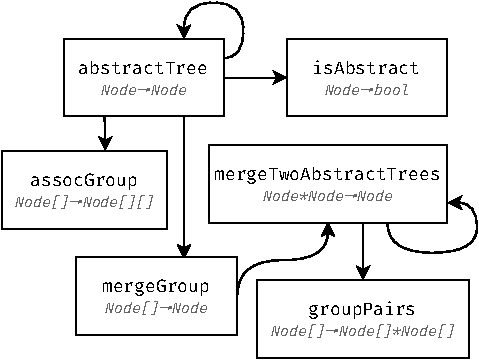
\includegraphics[width=0.7\linewidth]{appstract/explanations/functions_relations}
  \caption{Key functions involved in the \emph{abstractTree} algorithm. A directed arrow from function $f$ to $g$ indicates that $f$ calls $g$.}
  \label{fig:functions_relations}
\end{figure}

\begin{figure*}[]
  \centering
  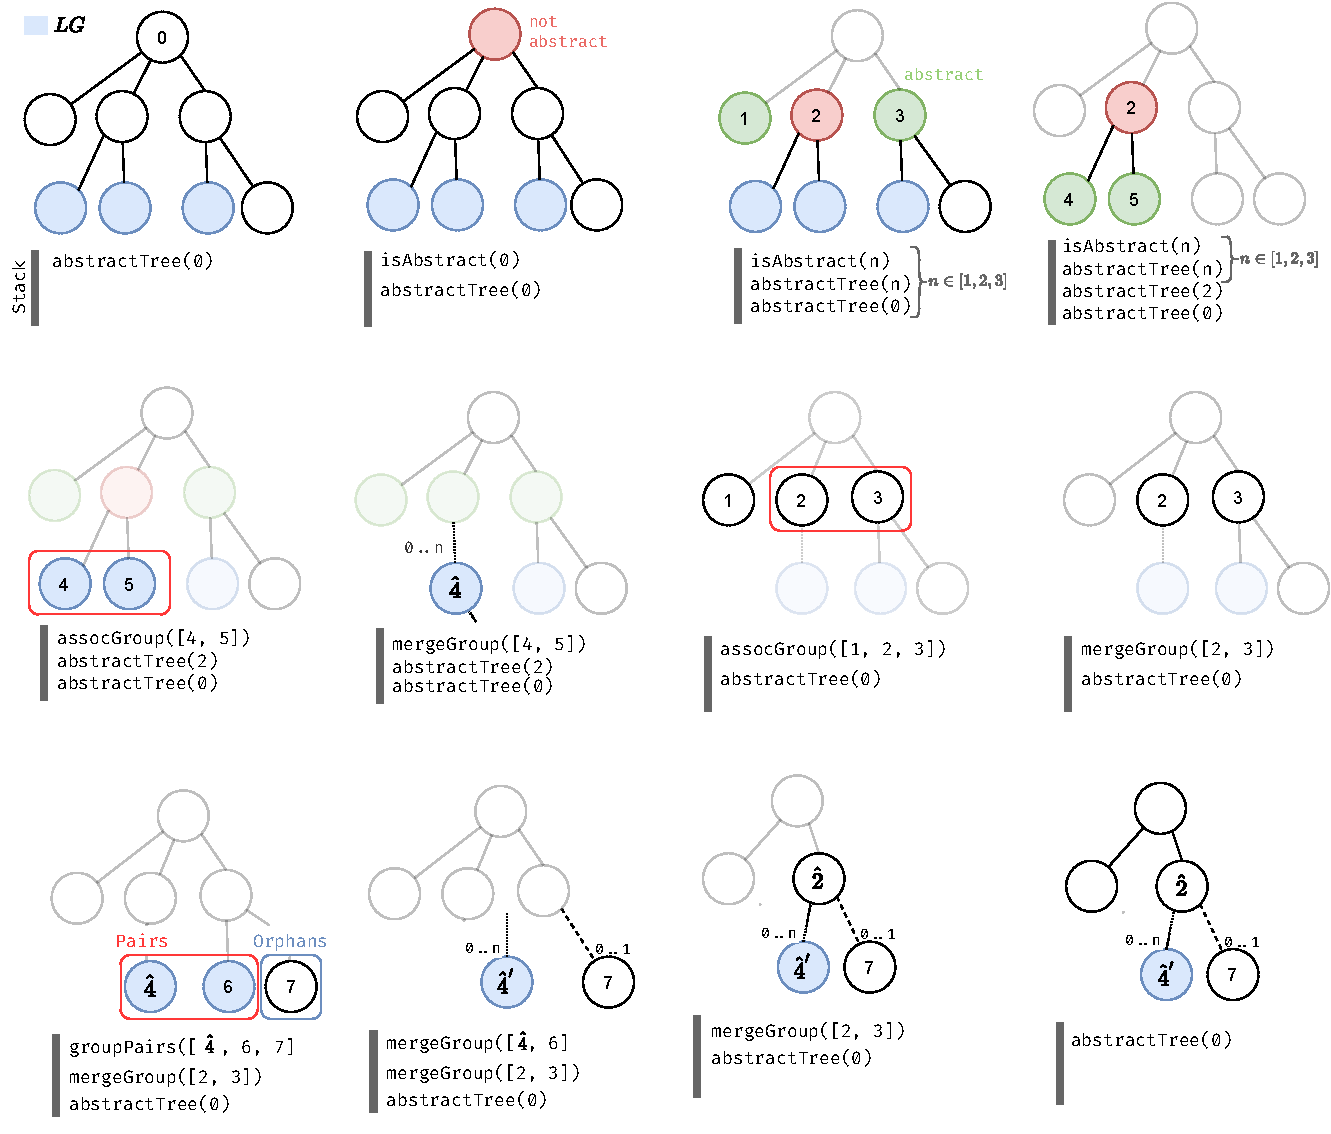
\includegraphics[width=0.8\linewidth]{appstract/explanations/steps_abstractTree}
  \caption{An example application of the \emph{abstractTree} function. For each figure, the stack of the current step is shown below.}
  \label{fig:steps_abstractTree}
\end{figure*}

Figure~\ref{fig:steps_abstractTree} describes an example application of the \emph{abstractTree} function.
At each step, the current stack of functions is shown at the bottom.
All functions shown have been described in the previous sections.
Figure~\ref{fig:functions_relations} summarizes all these functions and how they interact.
For simplicity, however, the \emph{mergeTwoAbstractTrees} is not explicitly mentioned, it is considered as part of the function \emph{mergeGroup}.

% \subsubsection{Complexity}

% \subsubsection{Coordinate System}
% When abstracting, in addition to the application abstraction $A$, we also build a coordinate system to locate each abstracted instance element.
% To build our coordinate system, we define the concept of \emph{box}.

% \begin{defn}{Box}
% We call a \textit{box} and we note $\hat{b} \in \hat{A}$ any template element that have a zero to many relationship with their parent.
% \end{defn}

% Every box is associated with a subset of several leaf groups

% \emph{Example:}
% ++++Create a figure that shows what a box is.

% Boxes are particularly interesting because they represent record containers. As such, they can be used as a useful anchor point to define a coordinate system allowing to locate instances of element templates.

% Let us consider a website containing a list of products. Each product contains a name and a price.
% After abstraction, product names and prices are mapped respectively to the template elements $\hat{e}_{name}$ and $\hat{e}_{price}$.

% Given an input element $e \in p$, the intra-page abstraction allows us to return the corresponding element $T_e(e)$ which means, in our example, either $\hat{e}_{name}$ or $\hat{e}_{price}$. But what if the user of \textsc{\appstract{}} needs to know which product was clicked on specifically?

% We build a \emph{coordinate system} allowing us to locate the instances of any template concerning their boxes.

% Two approaches are considered:
% \begin{enumerate}
%     \item Complete: coordinates depend on all boxes in the root-to-node path
%     \item Simplified: coordinates depend on the best box selected
% \end{enumerate}

% \emph{Examples.}
% ++++ Coordinates of the examples elements

% A complete coordinate system yields more information but is harder to take advantage of.
% The simplified approach has three main benefits: 
% \begin{enumerate}
% \item The coordinate system is simpler to use because it contains a fixed number of components
% \item Since there are overall fewer components, more elements will share the same coordinate reference (box).
% \item The box choosing process acts as an important filter for noise
% \end{enumerate}

% \paragraph{Box Choosing as a filter for noise}
% +++ Describe what kind of noise we can have (example: several elements with the same paths and they are a cluster, then one element with the same path but not a cluster)


% \paragraph{Choosing the best box}
% We study the cases where a Leaf-group is the offspring of several boxes (at different depths).

% Figures.... show some examples.

% Our observation leads us to think that in the majority of cases, a human would not consider all these boxes as valid record containers (for ex....) 

% This observation comes from the fact that in general, it is not super user-friendly to expose the user to nested layers of high variability.

% Choosing one only box allows to
% \begin{inparaenum}
%     \item provides more simple abstractions where many elements have the same coordinate base.
% \end{inparaenum}
% That's why we choose to select the best box.

% A "good" box follows the following:
% \begin{itemize}
%     \item It has many instances
%     \item ...
% \end{itemize}

% Voting mechanism:
% \begin{enumerate}
%     \item Each instance $e$ of each leaf-group $LG$ gives one vote for each box on its path.
%     \item Only box templates that account for more than a certain threshold of instances are considered. 
%     \item 
% \end{enumerate}

% \subsubsection{Intra-page abstraction as a Record extractor}
% If we restrict the original (non-abstracted) tree to boxes and text nodes, we get 

% \subsubsection{The algorithm}
% \paragraph{Merging two nodes}

% \subsubsection{Enrich \appstract{}ion}
% In this section, we study how to further enrich the abstraction inferred by \appstract{}.

% To understand the need for this stage, let us consider the case of a navigation menu containing a set of four links to different sections of the website: home page, products, blog, and contact.
% In this situation, it is very likely that the four menu links will be abstracted into one single template link $\hat{e}_{menu link}$.
% Unfortunately, the fact that all menu links are matched to a single template element may be problematic: if \textsc{\appstract{}} is used to monitor users' activity, then all clicks on the menu will be assimilated to 

\subsection{Inter-Page Abstraction}\label{appstract:sec:inter}
We described how to detect and abstract the repeating patterns contained within one page. 
In the second part of the \textsc{\appstract{}} approach, we detect and abstract repeating patterns across pages of the web application.

The inter-page abstraction relies on tree-matching.
A tree matching solution allows matching two web page DOM trees $p$ and $p'$. 
The matching $M_{p, p'}$ obtained is a subset of  $p \times p'$ such that each tuple $(e, e') \in M_{p, p'}$ represents the fact that the element $e \in p$ matches with the element $e' \in p'$ (e.g. $e$ and $e'$ contain the names of two different products on two different product pages $p$ and $p'$).

As described in Section~\ref{appstract:sec:overview}, inter-page abstraction is used at both the learning and prediction phases. In both cases, the inter-page abstraction can be described as a function that:
\begin{enumerate}
    \item takes two templates as input: the reference template and a new template,
    \item returns a template in which every template element $\hat{e}$ of the new template references its corresponding template element $\hat{e'}$ in the reference template (if a match was found).
\end{enumerate}

\begin{algorithm}
    \caption{Inter-page abstraction}\label{appstract:alg:inter-page}
    \begin{algorithmic}[1]
      \Function{inter}{$\langle p_{ref}, T_{ref} \rangle, \langle p, T \rangle$}
          \State $M \gets$ tree-matching($p$, $p_{ref}$)
          \State $T_{new} \gets$ T.map(($e$, $id$) $\to$ $T_{ref}[M[e]]$ if $e$ in $M$ else $id$)
          \State \Return $\langle p, T_{new} \rangle$
      \EndFunction
    \end{algorithmic}
\end{algorithm}

Algorithm~\ref{appstract:alg:inter-page} describes the inter-page abstraction process.
The function role is to create a new identifier map $T_{new}$ in which each element from $p$ maps to the id of the matching element in $p_{ref}$ (if there is any) or remains the same.

Figure~\ref{fig:appstract_overview} describes how the function \emph{inter} is used for both learning and prediction:
\begin{compactenum}
    \item during learning, we apply inter-page abstraction between the mother template and each of the other templates. This step allows for building a model of the application where elements that appear in all page templates will have the same id,
    \item during prediction, inter-page abstraction is used to match all elements from an unseen page to the template elements of its matching template page.
\end{compactenum}

\section{Limits}
Modeling a whole application is a highly ambitious task.
We hope our work can help progress toward this goal, but we cannot claim that it already does.
Indeed, our current work has several limits, mainly:

\emph{Template Topology}
Real-life templates may have a much more complex structure than the one we assume:
\begin{enumerate}
\item there can be a tree-like structure with deeply nested templates,
\item there could be graph-like template structure (\emph{e.g.}, components).
\end{enumerate}
Our current \emph{appstraction} method does not allow us to infer such template topologies.

\emph{Mother Template Selection}
During the learning stage, we choose the mother template arbitrarily among the existing template pages.
This selection process assumes that all template pages have an equivalent amount of common parts.

\section{Evaluation}\label{appstract:sec:evaluation}
In this section, we describe the experiment we devised allowing us to evaluate \appstract{}.
The idea of the experiment is to consider several samples of DOM elements couples and manually judge if they are correctly labeled (should they have the same id?)

\subsection{Experiment}
We intend to measure over- and sub-abstraction rates of \appstract{}. 
Fundamentally, \appstract{} allows the creation of semantically rich, application-wide ids for elements on a webpage.
Where:
\begin{compactitem}
  \item \textit{Semantically Rich} means that two instances of the same template should have the same id
  \item \textit{Application-wide} means that on a given application instances of a template will have the same id regardless of the page
\end{compactitem}
There are two ways in which \appstract{} can fail:
\begin{compactitem}
  \item \emph{Over-abstraction}: Items have the same id even though they are not of the same type, or
  \item \emph{Sub-abstraction}: Items have different ids even though a human would assign them the same.
\end{compactitem}
To analyze the performance of \appstract{}, we thus propose to measure the rates of over- and sub-abstraction.
To do so, we developed a visual way to explore the web page abstractions created by \appstract{}.
Given an application $A$:
\begin{compactitem}
  \item We apply \appstract{} to $A$ thus obtaining an abstraction $\langle \hat{A}, T_{\hat{A}} \rangle$
  \item Open two pages $p_{a_1}, p_{a_2}$ that we assume to be instances from the same template $p_a$ (e.g. two product pages or two blog posts)
  \item Use $\langle \hat{A}, T_{\hat{A}} \rangle$ to get the id $T_{\hat{p}}(e) = \hat{e}$ of every element $e$ on both pages $p_{a_1}, p_{a_2}$
  \item Visually display the id $\hat{e}$ when the mouse hovers over an element $e$
\end{compactitem}
This method allows us to simply analyze the results of \appstract{}.

We separate our experiment into two parts:
\begin{inparaenum}
    \item Over-abstraction and
    \item Sub-abstraction
\end{inparaenum}

\subsubsection{Defining Measures}\label{sec_definition_measures}
After having described what we refer to as over-abstraction and sub-abstraction, in this section, we give formal definitions of these measures.
To do so, we formulate the experimental application of \appstract{} as a binary classification problem in which each couple of elements between two pages can either have the same locator or a different one.
We then define over-abstraction and sub-abstraction as complementary to the precision and recall of our binary classification problem.

Let us consider two pages $p_1$ and $p_2$ from the same application $A$.
We apply \appstract{} to $A$ and obtain the abstraction $\langle \hat{A}, T_{\hat{A}} \rangle$.
Then, we apply the abstract model to $p_1$ and $p_2$: 
\begin{align}
T_{\hat{A}}(\hat{p}_1) &= \langle \hat{p_1}, T_{\hat{p_1}} \rangle \\
T_{\hat{A}}(\hat{p}_2) &= \langle \hat{p_2}, T_{\hat{p_2}} \rangle
\end{align}

We formulate the experimental application of \appstract{} as a binary classification problem.
\begin{defn}[\em Ground Truth Binary Classification function $f$]
\begin{align}
f:  p_1 & \times p_2 \to [0, 1] \\
f(e_1, e_2) &= 1 \text{ if $e_1 \sim e_2$} \\
f(e_1, e_2) &= 0 \text{ otherwise}
\end{align}
where $e_1 \sim e_2$ means that $e_1$ and $e_2$ are instances of the same template element (e.g. a buy button on a product page) as judged by a human.
\end{defn}
$f$ is the ground truth of our experiment. In practice, in the experiment, we only know a small manually labeled sample of $f$.

\begin{defn}[\em Prediction function $\hat{f}$]
\begin{align}
f:  p_1 \times p_2 & \to [0, 1] \\
f(e_1, e_2) &= 1  \text{ if $T_{\hat{p_1}}(e_1) =  T_{\hat{p_2}}(e_2)$}\\
f(e_1, e_2) &= 0 \text{ otherwise}
\end{align}
\end{defn}
$\hat{f}$ is a guess made using \appstract{} predicting whether two elements should have the same locator.


\begin{defn}[\em Prediction function $\hat{f}$]
\begin{align}
f:  p_1 \times p_2 & \to [0, 1] \\
f(e_1, e_2) &= 1  \text{ if $T_{\hat{p_1}}(e_1) =  T_{\hat{p_2}}(e_2)$}\\
f(e_1, e_2) &= 0 \text{ otherwise}
\end{align}
\end{defn}
Given the above definitions, we can define the traditional precision and recall of our binary classification problem:
\begin{defn}[\em Binary Classification Measures]
\begin{align}
tp &=|\{e_1, e_2 \in p_1, p_2 / f(e_1, e_2) = \hat{f}(e_1, e_2) = 1\}| \\
fp &=|\{e_1, e_2 \in p_1, p_2 / f(e_1, e_2) = 0, \hat{f}(e_1, e_2) = 1\}| \\
fn &=|\{e_1, e_2 \in p_1, p_2 / f(e_1, e_2) = 1, \hat{f}(e_1, e_2) = 0\}| 
\end{align}
where $tp, fp$, and $fn$ stand for true positive, false positive, and false negative, and |S| is the cardinality of a set $S$.
\begin{align}
precision_{p_1, p_2}(\hat{f}) &= \frac{tp}{tp + fp} \\
recall_{p_1, p_2}(\hat{f})  &= \frac{tp}{tp + fn}
\end{align}
\end{defn}

Finally, we define over-abstraction and sub-abstraction as complementary measures of precision and recall:
\begin{defn}[\em Over-abstraction rate]
\begin{equation}
o_{p_1, p_2}(\hat{f})  = 1 - precision
\end{equation}
\end{defn}
\begin{defn}[\em Sub-abstraction rate]
\begin{equation}
s_{p_1, p_2}(\hat{f})  = 1 - recall
\end{equation}
\end{defn}

In the next section, we describe an empirical experiment allowing us to estimate the over-abstraction and sub-abstraction rates of predictions made by \appstract{}. 

\subsubsection{Experimental Protocol}
We devise an experimental protocol allowing us to evaluate the performance of \appstract{} on an application.
We separate the experiment into two parts: sub-abstraction and over-abstraction evaluations.
In both experiments, we manually label couples of DOM elements from two pages of the same application.
The idea is to estimate the precision and recall of the function $\hat{f}$ defined in section \ref{sec_definition_measures}.

\paragraph{Selecting couples of pages}
Given an application containing several pages, we need to select a subset of page couples on which we experiment.
There are two possibilities:
\begin{enumerate}
    \item Picking random couples
    \item Picking couples of pages that seem to belong to the same template
\end{enumerate}
We choose the second possibility because it provides more relevant data to evaluate.

In the rest of the section, we thus describe the evaluation process on a single couple of DOMs $(p, p')$ belonging to the same template of the same application to which we already applied \appstract{}. 
Formally, it means we use the functions $T_{\hat{p}}$ and $T_{\hat{p'}}$.

\paragraph{Over-abstraction}
Over-abstraction measures the precision of our algorithm: to how many couples of elements do we mistakenly assign the same id?
More formally:
\begin{equation}
o_{p, p'}(\hat{f}) = 1 - \frac{tp}{tp + fp}
\end{equation}
where $tp$ is the number of true positives and $fp$ is the number of false positives.

The objective of this part of the experiment is thus to estimate $tp$ and $fp$ given a couple of DOMs $(p, p')$.
Both $tp$ and $fp$ concern the subset of positive couples: the subset of DOM elements couple $(e, e') \in p \times p'$ such that $T_{\hat{p}} = T_{\hat{p'}}$.

To label true and false positives, we develop a script that, given two abstracted web pages $p, p'$:
\begin{enumerate}
\item Display $p$ and $p'$ side by side,
\item Highlights one element of each page that has the same id,
\item Offer a popup allowing the tester to manually choose between "Correct", "Wrong" or "Skip"
\end{enumerate}

This experiment allows to estimate the amount of true positives $tp$ ("Correct") and false positives $fp$ ("Wrong").
The "Skip" option is most useful in cases where the elements highlighted are not visible.
Results allow us to calculate an estimate of the over-abstraction $\hat{o_{p, p'}}(\hat{f})$

\paragraph{Sub-abstraction}
 Sub-abstraction measures the recall of our algorithm: how many elements should have the same id but not?
 More formally:
 \begin{equation}
s_{p, p'}(\hat{f}) = 1 - \frac{tp}{tp + fn}
\end{equation}
 To estimate sub-abstraction, we develop a script that, given two abstracted web pages $p, p'$:
\begin{enumerate}
\item Display $p$ and $p'$ side by side
\item Ask the user to select one element from each web page that should have the same id
\item Check if they indeed have the same id. If yes, increment the number of true positive $tp$ else increment the number of false negatives $fn$
\end{enumerate}

We do not disclose the results of the comparison to avoid influencing the following experimenter's choices.

% \paragraph{Building the Dataset}
% Since the labeling is done manually, we can only select a limited set of applications to experiment on.
% We try to choose applications belonging to different categories.

% \subsubsection{Limits}
% As mentioned in Section \ref{appstract:sec:introduction}, \appstract{} opens up many applications, notably in data extraction, analytics, or testing. However, testing \appstract{} indirectly through one of these applications will not provide the same level of precision as the more direct evaluation that we propose. For example, trying to extract data using \appstract{} requires a lot of additional work that is not directly linked to \appstract{} (e.g. separating menu items from data records).
% This is the reason why we chose to develop a dedicated evaluation protocol for \appstract{}.

\subsubsection{Preliminary Results and Limitations}
While we, unfortunately, did not have enough time to lead the described experiments quantitatively, our first tests of \appstract{} are promising but show some limitations, mainly related to Free Text detection.
We call \textit{Free Text}, portions of web pages containing text written and, more importantly, formatted by the user. The most significant example of free text is content written on forums or comment sections.  Comment editors on these websites often offer users the option to format (bold, italic, paragraphs...) their text. The formatting tags in free text introduce noise that is difficult to ignore for \appstract{}. Indeed, the main assumption used by \appstract{} to separate content from presentation (templates) is that web applications present a high variability of content (text) encoded in a limited amount of templates. In the case of free text, this assumption is false: the structure of the webpage defined through tags is partially written by the user which leads to the high variability of structure since, in this case, the structure is also part of the content. \appstract{} then mistakenly believes the formatting tags should be used to infer the template which can lead to unexpected results.
To solve the free-text limitation, we need to find a way to detect free text.

\section{Conclusion}\label{appstract:sec:conclusion}
We believe \appstract{}'s approach is an important and pioneering solution in two ways.

Firstly, we introduce the webpage abstraction problem independently to its traditional areas of application (e.g. web testing, data extraction, web analytics). We propose a formalization of the abstraction problem using the idea of robust and semantically-rich application-wide identifiers.

Secondly, we propose an abstraction approach combining intra- and inter-page abstraction to generate such identifiers. While both intra- and inter-page abstraction underlying techniques are akin to existing approaches in different research areas, to our knowledge, the idea to combine both to infer a web application abstraction is original.

The web application abstraction problem we described is very complex, mainly because of the high variety of existing modern web applications. Unfortunately, \appstract{} is not the off-the-shelf web application abstraction solution working on any application that we intended to develop. \appstract{} mainly suffers from a lack of quantitative evaluation benchmark and can be misled by Free Text sections (e.g. comment sections or forum posts). However, we hope it will serve as a starting point to developing new solutions for the web application abstraction problem.
